% !TeX root = ../tfg.tex
% !TeX encoding = utf8
%
%*******************************************************
% Introducción
%*******************************************************

% \manualmark
%\markboth{\textsc{Introducción}}{\textsc{Introducción}} 

\chapter{Introducción}

En los últimos años, el fenómeno del \emph{Deep Double Descent} ha surgido como un importante campo de interés en el aprendizaje automático. Mientras que la sabiduría tradicional del aprendizaje sugiere que, a medida que aumenta la complejidad del modelo, el error fuera de la muestra disminuye inicialmente hasta alcanzar un mínimo y, a continuación, aumenta de manera monótona debido al sobreajuste, formando la tradicional curva con forma de ``U''. Este concepto tradicional del aprendizaje automático, conocido como equilibrio entre sesgo y varianza difiere de las recientes observaciones obtenidas, que se cuestionan este punto de vista, especialmente en modelos de aprendizaje profundo, en los que puede producirse una segunda disminución del error fuera de la muestra y alcanzar un nuevo mínimo, formando una nueva curva en la gráfica del error de generalización que presenta dos descensos. Este novedoso descubrimiento pone en tela de juicio la sabiduría clásica sobre el tema y proporciona nuevas perspectivas a la hora de crear y entrenar los modelos.\newline

Este trabajo de fin de grado se centra en explorar el concepto del \emph{Deep Double Descent}, sus fundamentos teóricos y sus implicaciones para el aprendizaje automático moderno. Un área clave de interés es cómo este fenómeno se manifiesta en redes neuronales profundas, conocidas por su enorme complejidad en cuanto a número de párametros se refiere y su potencial de sobreajuste. A pesar de que los modelos de aprendizaje profundo han tenido gran éxito en diversas aplicaciones, como la visión por computador o el procesamiento de lenguaje natural, la curva del doble descenso aporta nuevos conocimientos sobre cómo estos modelos pueden llegar a generalizar en un régimen que ha sido vagamente estudiado y explorado: el régimen sobreparametrizado.\newline

La idea clave detras del fénomeno es la existencia de dos zonas de actuación del modelo claramente diferenciadas, la zona infraparametrizada y la zona sobreparametrizada. Sin embargo, formalizar esta idea es significativamente complejo, dado que los modelos profundos funcionan como ``cajas negras'', lo que hace que, a medida que aumenta su complejidad, resulte cada vez más difícil interpretar y obtener resultados precisos sobre su funcionamiento interno.\newline

Aunque cada vez hay más estudios abordando el fenómeno, muchos de ellos se centran en una perspectiva empírica del mismo, sin ofrecer una base teórica suficiente, mientras que otros sistematizan conceptos del fenómeno sin llegar a conclusiones prácticas. Con este trabajo buscamos cerrar la brecha entre la teoría y la práctica unificando explicaciones teóricas suficientemente rigurosas con ejemplos empíricos del mundo real con el objetivo de ofrecer una comprensión lo más completa posible del fenómeno.\newline


\section{Definición del problema}

\begin{figure}[h]
    \centering
    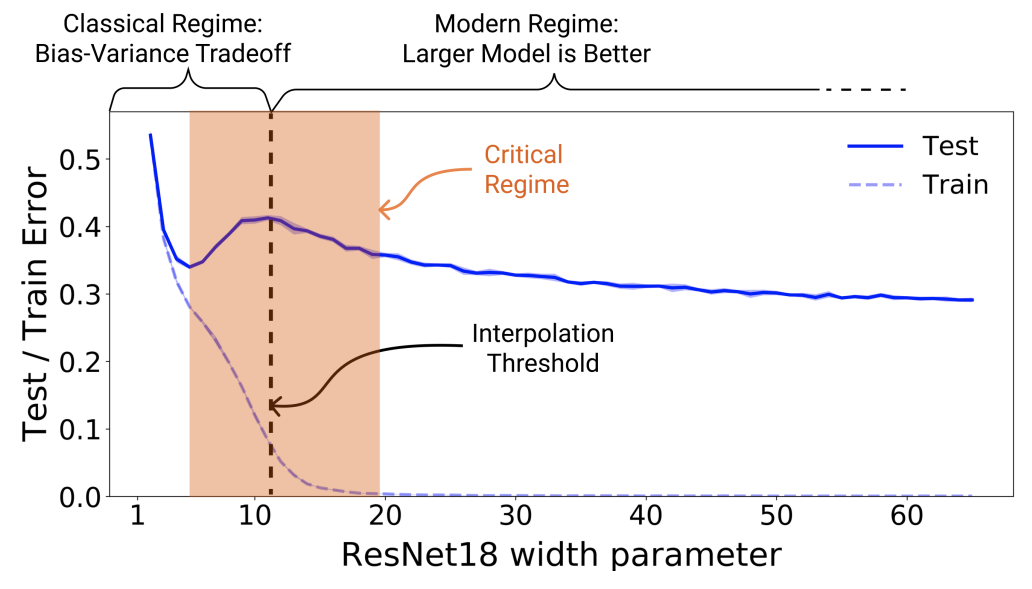
\includegraphics[width=\textwidth]{img/problem-definition.png}
    \caption[Ejemplo de doble descenso profundo en ResNet18~\cite{Nakkiran2019}.] {Ejemplo de doble descenso en ResNet18~\cite{Nakkiran2019}. La imagen muestra el error de entrenamiento (train error) y de generalización (test error) para la arquitectura ResNet18 con diferente capacidad (número de parámetros). En ella, observamos las tres regiones claramente diferenciadas, así como el máximo del error de generalización correspondiente al umbral de interpolación y los dos descensos de la curva de dicho error.}\label{fig:ejemplo-definicion-double-descent}
\end{figure}

El término \emph{doble descenso profundo (deep double descent,~\cite{Belkin2019})} describe la forma que toma la curva del error de generalización (error fuera de la muestra) de un modelo de aprendizaje como función de la capacidad del mismo. De manera intuitiva, podemos distinguir 3 zonas o regiones diferenciadas en dicha curva:

\begin{itemize}
    \item \textbf{Región clásica (infraparametrizada):} En esta región, el modelo no es capaz de capturar toda la complejidad subyacente de la distribución de los datos debido a su baja capacidad. Como resultado, el error de generalización disminuirá inicialmente, ligado al hecho de que el modelo aprende de los datos de entrenamiento. Sin embargo, llegado un momento, el error de generalización comenzará a aumentar de manera progresiva (véase \autoref{fig:ejemplo-definicion-double-descent}), dando lugar a la clásica curva en forma de ``U'' y ligado al hecho (tradicional) de que el modelo, en lugar de seguir aprendiendo de los datos y obtener patrones de los mismos, memoriza los datos de entrenamiento.

    \item \textbf{Región moderna (sobreparametrizada):} En esta región, el modelo tiene una capacidad mayor que la necesaria para ajustar los datos de entrenamiento, es decir, dispone de suficientes herramientas (parámetros) para ajustar cada uno de los datos de entrenamiento. Contrariamente a lo que se esperaría de forma clásica, el error de generalización no necesariamente aumenta en este región y, bajo ciertas condiciones, dicho error puede reducirse nuevamente, produciendo un nuevo descenso de la curva del error de generalización que se conoce por \emph{doble descenso}.
    
    \item \textbf{Región crítica:} Esta región marca la transición entre la región infraparametrizada y la región sobreparametrizada y engloba zonas de ambas regiones. Dentro de ella, se encuentra el llamado \textbf{umbral de interpolación}, que corresponde al punto donde el modelo tiene justo la capacidad suficiente para ajustar perfectamente los datos de entrenamiento (mismos parámetros que datos). En este punto crítico, el error de generalización alcanzará su máximo.\newline
       
\end{itemize}

Este doble descenso puede llegar a suponer la obtención de un nuevo mínimo en la curva del error de generalización, es decir, la obtención de modelos cuyas predicciones sean aún mejores. Sin embargo, se abre la puerta a la investigación del por qué ocurre este novedoso fenómeno, además de que tendremos que replantearnos algunas respuestas, tradicionalmente correctas, ante preguntas clásicas del aprendizaje profundo.\newline

\section{Motivación}

En el ámbito del aprendizaje automático, es de cultura general conocer la existencia de una brecha entre el desarrollo empírico y la fundamentación teórica subyacente. Los modelos modernos, en particular las redes neuronales profundas, han demostrado resultados sorprendentes~\cite{Sejnowski2020TheUE, He2020RecentAI} desde la generación de imágenes realistas mediante redes generativas hasta el procesamiento de lenguaje natural (\textit{Natural Language Processing, NLP}). Sin embargo, estos resultados se logran sin una comprensión teórica completa~\cite{Ben-David2009}, especialmente debido al hecho de la facilidad de obtener resultados suficientemente decentes a través de la experimentación, sin la preocupación de preguntarnos si lo que realmente estamos probando es verdaderamente lo más eficiente o adecuado para alcanzar los mejores resultados posibles.\newline

Esta capacidad para obtener resultados que consideramos satisfactorios ha llevado a un enfoque predominantemente práctico, donde los avances se producen de manera más rápida a través del ensayo y error que mediante modelos matemáticos bien fundamentados, lo que impide comprender, desde una perspectiva teórica, tanto la eficacia como las verdaderas limitaciones que estos modelos podrían alcanzar. Este fenómeno plantea cuestiones sobre la sostenibilidad de este enfoque práctico y la necesidad de desarrollar un marco teórico que permita anticipar y guiar estos avances en lugar de simplemente reaccionar ante ellos.\newline

Debido a esta desconexión entre los avances teóricos y empíricos, han comenzado a surgir discrepancias y fenómenos no esperados en los resultados modernos, en particular en los que a modelos profundos se refiere. Es aquí donde se enmarca el concepto del \emph{Deep Double Descent}, fenómeno por el cual, a través de resultados prácticos, se ha corroborado como la práctica continúa superando las expectativas teóricas tradicionales y por el que hoy en día surgen numerosas líneas de estudio tratando de dar una explicación al respecto, resaltando como la teoría subyacente aún está vagamente desarrollada.\newline

De igual manera, este fenómeno tiene una relevancia crucial, ya que podría transformar la forma en que se diseñan y optimizan los modelos profundos. Tradicionalmente, el enfoque clásico sugiere que, a medida que se aumenta la complejidad del modelo, este tendía a sobreajustarse a los datos, lo que limitaba su capacidad de generalización, lo que impulsaba a optar por modelos más simples. Sin embargo, con este fenómeno, se ha demostrado que, más allá del sobreajuste, los modelos no solo dejan de aumentar su capacidad de generalización, sino que incluso mejoran, alcanzando una generalización aún mejor a la inicial. Este descubrimiento sugiere que, siguiendo este enfoque, podríamos centrarnos en desarrollar modelos más complejos sin necesidad de aplicar técnicas de regularización para evitar el sobreajuste, lo que nos permitiría obtener mejores resultados.\newline

En conclusión, el fenómeno del \emph{Deep Double Descent} representa un cambio de paradigma, digno de estudio, en el aprendizaje automático. Comprender los principios subyacentes no solo nos permitiría avanzar en nuestra comprensión teórica del aprendizaje automático, sino que también ayudaría a ir cerrando la brecha entre la teoría y la práctica. De hecho, si se logra desarrollar un marco teórico sólido, sería posible guiar la creación y optimización de modelos, haciendo que los avances prácticos sean más predecibles.\newline

\section{Objetivos}

El objetivo principal de este TFG radica en tratar de ofrecer una explicación detallada y estructurada del novedoso fenómeno \emph{Deep Double Descent}. Este estudio se centrará en proporcionar una visión actualizada y rigurosa de sus fundamentos teóricos, implicaciones prácticas y relevancia en el desarrollo de modelos modernos, asegurando que el contenido se mantenga en concordancia con los avances más recientes en la investigación.\newline

Para alcanzar este objetivo, se han definido dos líneas de trabajo interrelacionadas: una orientada al desarrollo \textbf{matemático} y otra enfocada en la parte \textbf{informática}. Ambas líneas se desarrollan de manera conjunta y complementaria, de modo que los avances teóricos guían y fundamentan la implementación práctica, mientras que los resultados experimentales permiten validar y enriquecer la comprensión teórica. A su vez, cada una de estas líneas de trabajo se descompone en una serie de objetivos parciales que, en conjunto, guían el desarrollo del proyecto.\newline

\subsection{Objetivo matemático}

El objetivo fundamental para la parte matemática consiste en profundizar en la comprensión teórica del \textit{Deep Double Descent} a través del estudio detallado de sus fundamentos matemáticos, explorando las relaciones con conceptos clásicos como el equilibrio sesgo-varianza y su posible conexión con la teoría de la aproximación no lineal. Con el fin de abordar de forma sistemática las distintas fases de este análisis, el presente objetivo se descompondrá en los siguientes objetivos parciales:

\begin{itemize}
    \item Realizar un análisis exhaustivo y detallado del estado del arte, revisando las principales teorías, descubrimientos y avances matemáticos relacionados con el fenómeno.
    \item Explicar de manera detallada la sabiduría clásica relacionada con el tema, analizando las teorías y enfoques tradicionales que prevalecen en la literatura, estableciendo las bases necesarias para entender el fenómeno.
    \item Investigar y analizar el fenómeno del \textit{Deep Double Descent}, proporcionando una explicación detallada de sus fundamentos y explorando en profundidad los hallazgos más relevantes de la literatura científica sobre el tema.
    \item Adentrarnos en la teoría de la aproximación no lineal con el propósito de identificar y analizar posibles analogías con el fenómeno, explorando cómo los enfoques no lineales pueden ofrecer una comprensión más profunda y enriquecedora de las dinámicas que subyacen a este fenómeno.\newline
\end{itemize}

\subsection{Objetivo informático}

El objetivo esencial para la parte informática consiste en llevar a cabo la constatación experimental del fenómeno mediante la implementación y análisis de diversas arquitecturas que permitan validar y estudiar empíricamente su comportamiento. Esta parte experimental busca no solo ilustrar la aparición del fenómeno en distintos escenarios y arquitecturas, sino también corroborar y complementar los resultados obtenidos en la parte matemática, estableciendo así una conexión sólida entre la teoría y la práctica. Con el fin de abordar de forma sistemática las distintas fases de este análisis, el presente objetivo se descompondrá, al igual que el objetivo de la parte matemática, en los siguientes objetivos parciales:

\begin{itemize}
    \item Realizar un análisis exhaustivo y detallado de los casos prácticos y representaciones experimentales en los que se ha manifestado el fenómeno, revisando los principales comportamientos y patrones.
    \item Presentar resultados experimentales que validen los desarrollos teóricos realizados en la parte matemática, demostrando la coherencia con las predicciones teóricas.
    \item Desarrollar un análisis experimental que respalde la aparición y las características del fenómeno, proporcionando evidencias prácticas que contribuyan a una comprensión más profunda de su comportamiento en diferentes modelos y escenarios en los que puede aparecer.\newline
\end{itemize}

\section{Planificación del proyecto}

\endinput
